%Please use LuaLaTeX or XeLaTeX
\documentclass[11pt,aspectratio=169]{beamer}

\usepackage[ngerman]{babel}
\usepackage{ragged2e}

\definecolor{ethblue}{RGB}{32, 91, 174}
\definecolor{mygrey}{RGB}{175, 175, 175}

\hypersetup{
  colorlinks=true,
  urlcolor=ethblue,
  linkcolor=ethblue,
  citecolor=ethblue
}

\title{Theoretische Informatik}
% \date[ABC 2021]{24. Sep 2026}
\date[]{15. Okt 2026}
\author{Olivér Kovács}
% \institute{Organizational Unit\\can spread over 2 lines}

\usetheme{eth}

\colorlet{titlefgcolor}{ETHBlue}
\colorlet{accentcolor}{ETHRed}

\begin{document}

%\def\titlefigure{elements/title-page-image}		% Default image
%\def\titlefigure{elements/title-page-image-43}	% Use this for 4:3 presentations

\titleframe

% \tocframe

% \section{Layout}

\begin{frame}{Organisatorisches}
    \begin{itemize}
        \item Midterm: Fr, 6. Nov 2026 16-18 Uhr
        \item Endterm: Fr, 11. Dez 2026 16-18 Uhr
    \end{itemize}
\end{frame}

\begin{frame}{Serie Aufgabe 6}
    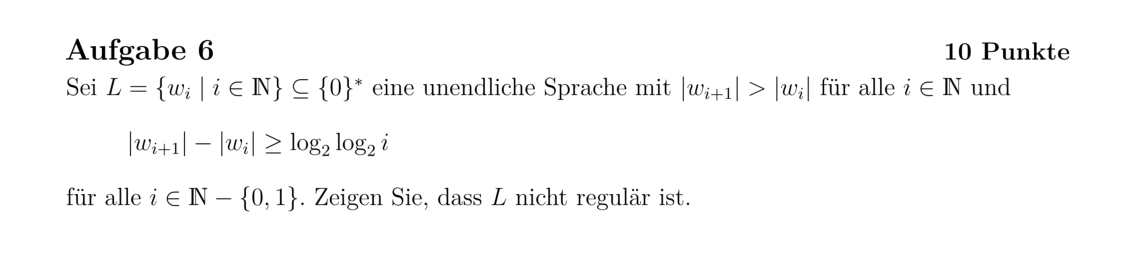
\includegraphics[width=32em]{img/a6}
\end{frame}

\begin{frame}{Quiz Frage 1}
    Seien \(L_1, L_2\) zwei nichreguläre Sprachen über demselben Alphabet.
    Sind die folgenden Sprachen immer, manchmal, oder nie regulär?

    \begin{enumerate}
        \item \(L_1^{C}\)
        \item \(L_1 - L_2\)
        \item \(L_1 \cup L_2\)
        \item \(L_1 L_2\)
    \end{enumerate}
\end{frame}

\begin{frame}{Nichtdeterminismus}
    \textbf{Satz 3.2.} Zu jedem NEA \(M\) existiert ein EA \(A\),
    so dass \(L(M) = L(A)\).
\end{frame}


\begin{frame}{Wie zeigt man Minimalität?}

Sei \(L\) eine reguläre Sprache.
Wir wollen beweisen, dass jeder EA \(A\) mit
\(L(A) = L\) mindestens \(n\) Zustände hat.

\vspace{2em}

\textbf{Idee:} Verwende Lemma 3.3.

\begin{itemize}
    \item Finde \(n\) verschiedene Wörter \(w_1, \ldots, w_n\).
    \item Finde für alle \(i \neq j\) ein Suffix \(z\), so dass gilt
        \[
            w_i z \in L \iff w_j z \not\in L .
        \]
\end{itemize}

\end{frame}

\begin{frame}{Turingmaschine}

\textbf{Definition 4.1.}
Eine \textit{Turingmaschine (TM)} ist ein 7-Tupel
\(M = (Q, \Sigma, \Gamma, \delta, q_0, q_{\text{accept}}, q_{\text{reject}})\).
Dabei ist

\begin{itemize}
    \item \(Q\) die \textit{Zustandsmenge} von \(M\),
    \item \(\Sigma\) das \textit{Eingabealphabet},
    \item \(\Gamma\) das \textit{Arbeitsalphabet},
    \item \(\delta : (Q - \{q_{\text{accept}}, q_{\text{reject}}\}) \times \Gamma
        \to Q \times \Gamma \times \{L, R, N\}\) die \textit{Übergangsfunktion},
    \item \(q_0 \in Q\) der \textit{Anfangszustand},
    \item \(q_{\text{accept}} \in Q\) der \textit{akzeptierende Zustand},
    \item \(q_{\text{reject}} \in Q\) der \textit{verwerfende Zustand}.
\end{itemize}

\end{frame}

% \setbeamertemplate{footline}{}

\begin{frame}{Aufgaben}
    \begin{enumerate}
        \justifying
        \item \textbf{Aufgabe 1.}
            Beweise, dass jeder DEA, der die Sprache
            \[
                L_1 = \{w \in \{a, b\}^* \mid w \text{ enthält } ab \text{ gleich of wie } ba\}
            \]
            akzeptiert, mindestens 5 Zustände hat.
        \item \textbf{Aufgabe 2.}
            Konstruiere einen NEA mit höchstens 4 Zustände, der
            \[
                L_2 = \{w \in \{a, b, c, d\}^* \mid w \text{ enthält mindestens eines der Teilwörter } ab, bc, adc\}
            \]
            akzeptiert.
        \item \textbf{Aufgabe 3.}
            Konstruiere mittels Potenzmengenkonstruktion einen EA für \(L_2\).
        \item \textbf{Aufgabe 4.}
            Beschreibe informell eine TM, welche immer hält und die Sprache
            \(L_4 = \{a^{n^2} \mid n \in \mathbb N \}\) akzeptiert.
    \end{enumerate}
\end{frame}

\end{document}
